% TODO: 

% five figure vs. six figure salary (compare with $5 vs $6 average tip)
% Democratic presidential candidate example
%          New Zealand example (archive.stats.govt.nz/infoshare,
%              Tourism > International Travel and Migration > Visitor 
%                  Arrival Totals (Monthly)
%                  (see nz.py and nz.csv in teaching/219)
%
% exponential vs. power-law; "fat tails" "scale-free"
%     exp_vs_power.py
%     expected value of exp, and power-law...doesn't exist!
%
% Scott Page's insight: you get normal distro when you have a bunch of
% *independent* events that are added up or averaged (Central Limit Theorem),
% and you get a power-law when you have a bunch of *dependent* events that are
% added up or averaged (like preferential attachment, among other examples.)
%
% animal example

\chapter{Using logarithms}

\index{logarithms}

Recall that the logarithm is the inverse operation of exponentiation. What is
$10^3$? 1,000. So what is the log of 1,000? 3. It's really that simple.
Instead of asking, ``what is ten to this particular power?'' I'm asking ``what
power would I raise 10 to in order to get this particular number?''

(This is assuming we're using ``base-10 logarithms,'' notated as
$\log_{10}$. You can use any other base as well: common choices are 
2 (sometimes $\log_{2}$ is abbreviated ``$\lg$''),
$e$ ($\log_{e}$, the ``natural'' logarithm, is usually abbreviated ``$\ln$''),
and 10 ($\log_{10}$ is often just plain ``$\log$''.))

The role of the logarithm is to mercilessly crush numbers down to size.

\begin{center}
\HeaderRows{1}   % x / log x header row
\begin{tabular}{c|c}
$x$ & $\log x$ \\
\hline
1 & 0 \\
10 & 1 \\
100 & 2 \\
1,000 & 3 \\
10,000 & 4 \\
100,000 & 5 \\
... & ... \\
\end{tabular}
\end{center}

Enormous numbers -- in the millions -- get squished down to single digits, and
\textit{the squashing gets more dramatic as the size of the number grows}.
Jumping from 1 to 10 (a difference of 9) netted us one higher in terms of
logarithm, but jumping from 10 all the way to 100 (a difference of
\textit{90}) \textit{also} only got us one higher. It's this property that
makes logarithms useful.

\index{order of magnitude}

Another way to think of logarithms is ``the logarithm of $x$ is the order of
magnitude of $x$.''

One property of logarithms that is extremely important to know is this:
\begin{align*}
\log(xy) = \log(x) + \log(y)
\end{align*}

Thus logarithms effectively \textit{turn multiplications into additions}. One
practical implication of this truth is leveraged in natural language
processing systems: we often find ourselves multiplying minuscule quantities
(very close to zero). As we multiply these, we get closer and closer to zero,
and eventually Python doesn't have enough precision to even represent a number
that low. But by dealing with logarithms, we're adding instead of multiplying
and avoid that problem completely.

A natural consequence of the above property is this one:
\begin{align*}
\log(x^a) = a \log(x)
\end{align*}

\section{Logarithmic plots}

\index{semi-log plot}
\index{log-log plot}

A common plotting technique is to use not the raw values of the independent
variable on the $x$ axis, but rather their logarithms. If we do this, we have
a \textbf{semi-log plot}. If we do this for both the $x$ and the $y$ axis, we
have a \textbf{log-log plot}.

Why would we do this? There are three reasons:
\begin{enumerate}
\itemsep1em
\item \textbf{It reins in large variations in the data.} If some of our data
points are orders of magnitude larger than others, the detail of the smaller
points gets completely swamped in trying to plot the larger points. Plotting
orders-of-magnitude instead of raw values solves this problem, though you have
to remember you did this when interpreting the plot!

\index{celebrities}
\index{UK}

Here's a (fictitious) example of some American and British celebrities, and
their total Instagram ``likes'':
\begin{Verbatim}[fontsize=\footnotesize,samepage=true,frame=single,framesep=3mm]
plt.plot(uk, linestyle='None', color="red", marker=".",
    label="UK")
plt.plot(us, linestyle='None', color="green", marker=".",
    label="US")
plt.legend()
plt.show()
\end{Verbatim}

\begin{figure}[ht]
\centering
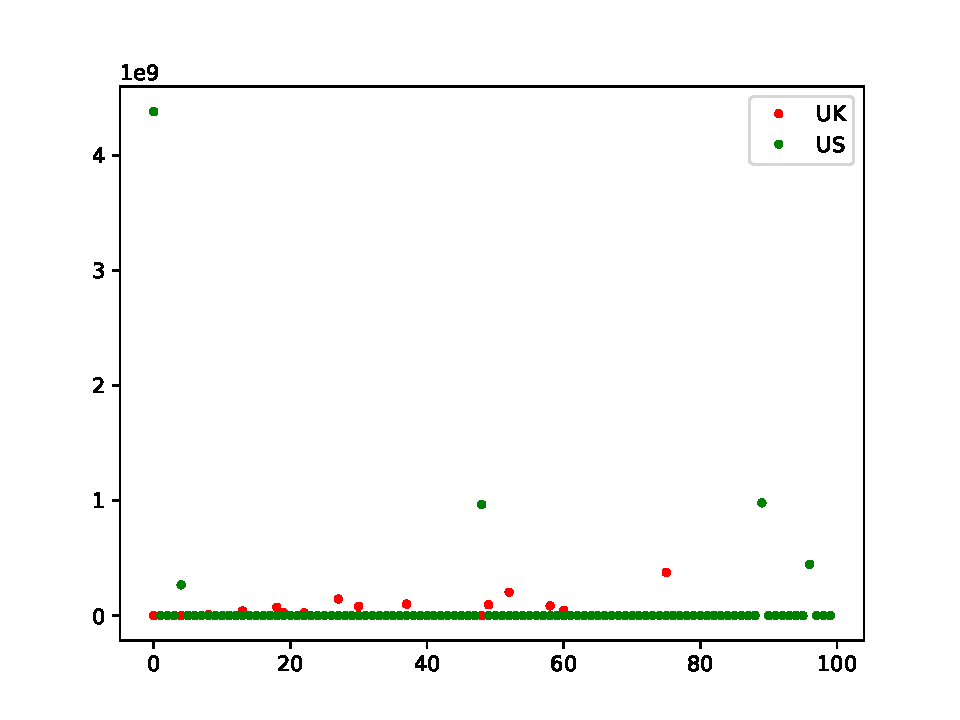
\includegraphics[width=1\textwidth,
  alt={Scatter plot of total Instagram likes for 100 celebrities, red dots for UK and green for US, on a linear vertical axis up to 4.4 billion. Nearly every point sits on the zero line; one US celebrity at the far left reaches 4.4 billion, two US points sit near 1 billion, and a handful of UK and US points lie between 0.1 and 0.5 billion.}]{rein1.pdf}
\caption{A regular (non-logarithmic) plot of celebrity ``likes.''}
\label{fig:rein1}
\end{figure}

The scatterplot is shown in Figure~\ref{fig:rein1}. It has limited use,
because there are a few uber-celebrities (Justin Bieber, \textit{etc.}) who
have far more ``likes'' than anyone else. Hence most people are crushed
against the bottom of the plot and we can't (say) compare the UK people with
the US people easily.

\index{scatter plot!logarithmic scale}

We can dramatically improve the readability and analyze-ability by plotting
the $y$ axis on a log scale. Just add this line before \texttt{plt.show()}:
\begin{Verbatim}[fontsize=\small,samepage=true,frame=single,framesep=3mm]
plt.yscale('log')
\end{Verbatim}

and voila, Figure~\ref{fig:rein2}. It's imperative that when you do this,
however, you remember that the $y$-axis no longer represents number-of-likes,
but log-number-of-likes.

\begin{figure}[ht]
\centering
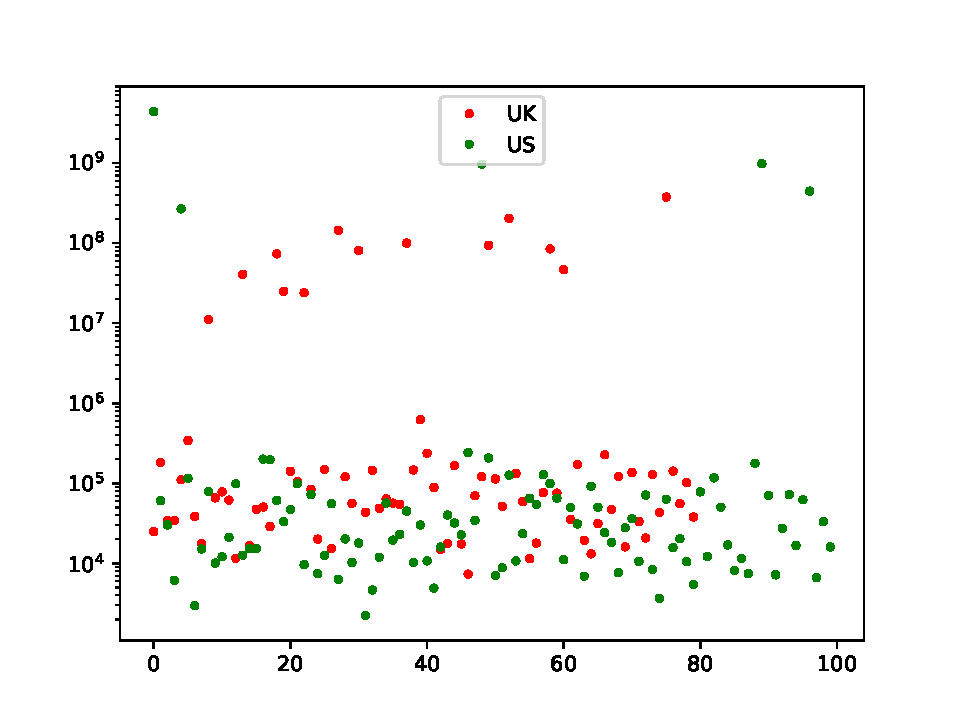
\includegraphics[width=1\textwidth,
  alt={The same celebrity likes on a logarithmic vertical axis from ten thousand to ten billion. The points now spread into a wide band mostly between ten thousand and a few hundred thousand likes, with about a dozen UK and US outliers between ten million and one billion, and the single US celebrity at about 4 billion at the top.}]{rein2.pdf}
\caption{A logarithmic plot of the same data from Figure~\ref{fig:rein1}.}
\label{fig:rein2}
\end{figure}

\index{relative vs.~absolute changes}
\index{absolute vs.~relative changes}
\index{stock prices}
\index{Stephen, Inc.}

\item \textbf{A semi-log plot shows \textbf{relative} (multiplicative) changes
instead of \textbf{absolute} (additive) changes.} Consider
Figure~\ref{fig:stock1}, whose (ordinary, not logarithmic) plot depicts a
fictional company's stock price over time. Two significant events occurred in
this company's history: one in April 2015 and the other in March 2017. Both
caused the stock's value to jump. Question: would you rather have bought stock
immediately before event A and sold it immediately after, or done the same
before/after B?

\begin{figure}[ht]
\centering
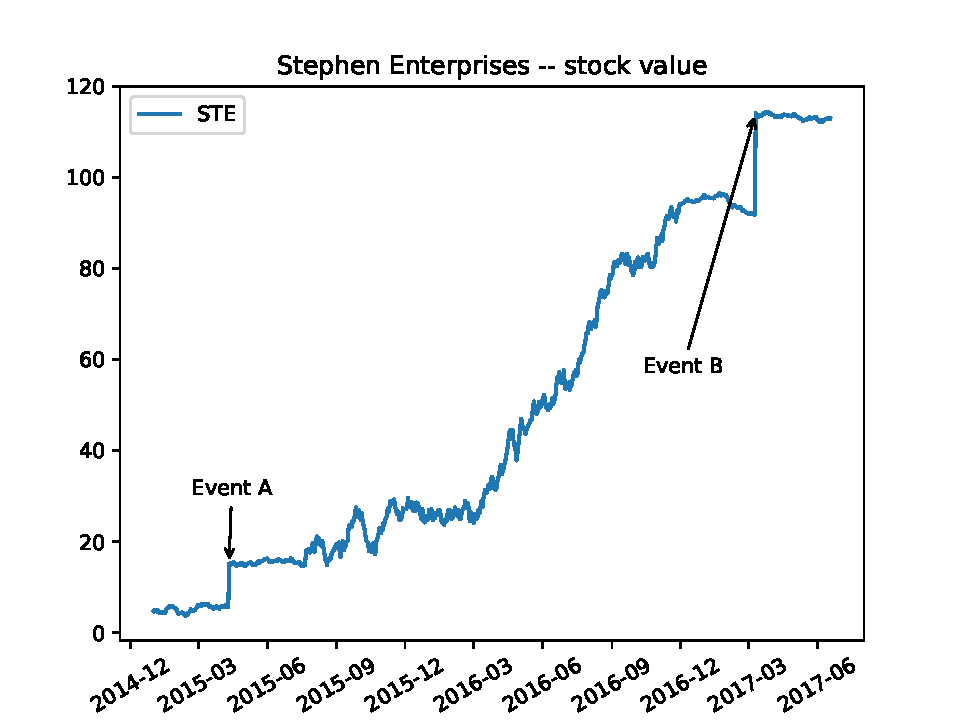
\includegraphics[width=0.8\textwidth,
  alt={Line plot titled Stephen Enterprises stock value, December 2014 to June 2017, price on a linear axis from 0 to 120. The line rises from about 5 to a plateau near 113. Two labeled jumps: Event A in early 2015 lifts the price from about 5 to 15, and Event B in early 2017 lifts it from about 92 to 113; between them the price climbs steadily through 2016.}]{stock1.pdf}
\caption{A regular (non-logarithmic) plot of a company's stock price.}
\label{fig:stock1}
\end{figure}

From Figure~\ref{fig:stock1}, it may look like event B is the better bet:
after all, it looks like the jump was higher. But this is an \textit{absolute}
distance: in other words, the total number of dollars per share jumped higher
for event B. But for something like an investment, you actually don't care
about this absolute number, but the \textit{relative} number. 

Look carefully at event A: before the jump, the stock was selling at about \$5
per share, and afterwards, at about \$15. This means that if you timed this
right, you \textit{tripled your money}! (Buy \$1000 worth of stock in April
2015, and you sell it for \$3000 the following day.) Compared to event B, this
is a way better deal. Consider that at event B, the stock went from \$90 to
\$110. Sure, \$20 is more than \$10 in absolute dollar terms, but if you
bought \$1000 worth of stock in March 2017 and sold it the following day,
you'd have sold it for \$$1000 \times \frac{110}{90} = $\$1222. Nice, but not
nearly the windfall of event A.

\index{semi-log plot}
For this reason, stocks and other investments are nearly always shown on a
semi-log plot, like the one in Figure~\ref{fig:stock2}. it has the advantage
that \textit{same-size increases on the (log) $y$ axis correspond to identical
\textit{relative} (multiplicative) increases of the stock.} In other words, if
the stock rises an inch somewhere on the plot, and it rises an inch somewhere
else, these represent equal gains for investors \textit{no matter how high the
stock value is in absolute terms.} Such is the magic of logs.

\index{windfall}

In this example, you can easily see from the semi-log plot that event A was a
bigger windfall for investors than event B.

\begin{figure}[ht]
\centering
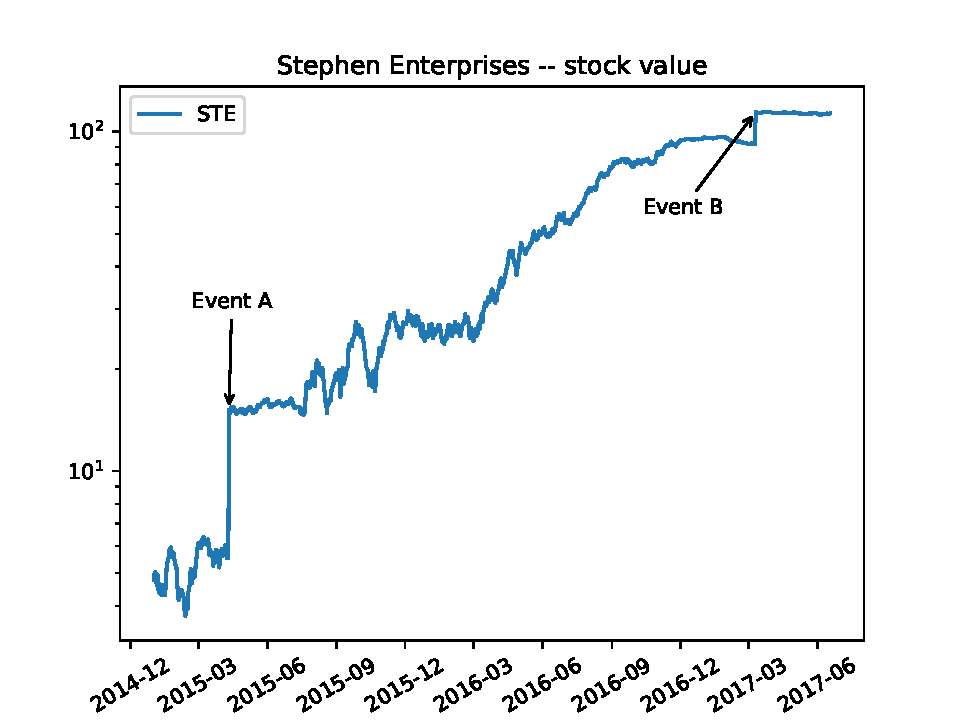
\includegraphics[width=0.8\textwidth,
  alt={The same stock price on a logarithmic vertical axis from about 5 to 120. The Event A jump in early 2015 now shows as the taller step, roughly tripling the price, while the Event B jump in early 2017 is a small step; the 2016 climb is a gentle upward curve.}]{stock2.pdf}
\caption{A semi-logarithmic plot of a company's stock price.}
\label{fig:stock2}
\end{figure}

\index{exponential relationship}
\index{power-law relationship}
\item \textbf{It reveals exponential and power-law relationships.} This
requires a little math to understand. Suppose we have two variables, $x$ and
$y$, and they are related according to something like this:
\begin{align*}
y = p \cdot e^{qx}
\end{align*}
where $p$ and $q$ are just numbers. For example,
\begin{align*}
y = 5.2 \cdot e^{2.96 x}
\end{align*}

Now if we plot $x$ vs $y$ on a standard plot, we get a curvy exponential
function that is very difficult for the human eye to distinguish from other
curvy functions. But suppose we plot not $y$, but the \textit{logarithm} of
$y$? 

Let's take the natural log ($\ln$) of both sides of the equation. Using our
properties from above, we get:

\begin{align*}
\ln y &= \ln (5.2 \cdot e^{2.96 x}) \\
&= \ln(5.2) + \ln(e^{2.96 x}) \\
&= 1.649 + 2.96 x \\
\end{align*}
This is just a linear equation with a slope ($m$) of 2.96 and a $y$-intercept
($b$) of 1.649. So plotting this relationship on a semi-log plot will give us
a straight line.

\index{rate of increase}

Why do we care? Because it turns out that exponential relationships like this
come up a lot in the world. One ubiquitous pattern is that of exponential
growth or decay: any time that \textit{the rate of increase of a quantity}
(like the number of new baby rabbits added to a rabbit population) is
proportional to \textit{the quantity itself} (the number of existing rabbits),
we have exponential growth. And any time that the rate of \textit{de}crease of
a quantity (like the number of mechanical parts that wear out) is proportional
to the quantity itself (the total number of mechanical parts owned by the
company), we have exponential decay.

\index{power-law relationship}
Another important kind of relationship is often mistaken for exponential
growth, but is emphatically \textit{not}. It's called a ``power-law''
relationship, and has caused much buzz in the scientific community over the
past decade or so. It occurs when we have a simple polynomial relationship:
\begin{align*}
y = p \cdot x^{q}
\end{align*}
where $p$ and $q$ are just numbers. For example,
\begin{align*}
y = 3.9 \cdot x^{-2.45}
\end{align*}

Again, some math: if we take the logarithm of both sides, we get:
\begin{align*}
\ln y &= \ln (3.9 \cdot x^{-2.45}) \\
\ln y &= \ln (3.9) + \ln (x^{-2.45}) \\
\ln y &= 1.361 -2.45 \ln (x) \\
\end{align*}
\normalsize

\vspace{-.25in}
If we plot not $y$ vs $x$, but $\ln y$ vs $\ln x$ (in other words, a
\textbf{log-log plot}, we will get a straight line. (You can see this by
mentally substituting your letter of choice for $\ln x$ and another letter of
your choice for $\ln y$. Now you have a plain old linear equation with a slope
of -2.45 and an intercept of 1.361.)

To see how the logarithmic plots reveal this, consider
Figure~\ref{fig:straightLines}, each of which is a plot of the same three
synthetic data sets. The blue points are linear in $x$, the red points are
exponential, and the green points are power-law (with an exponent of 6).

\begin{figure}[ht]
\centering
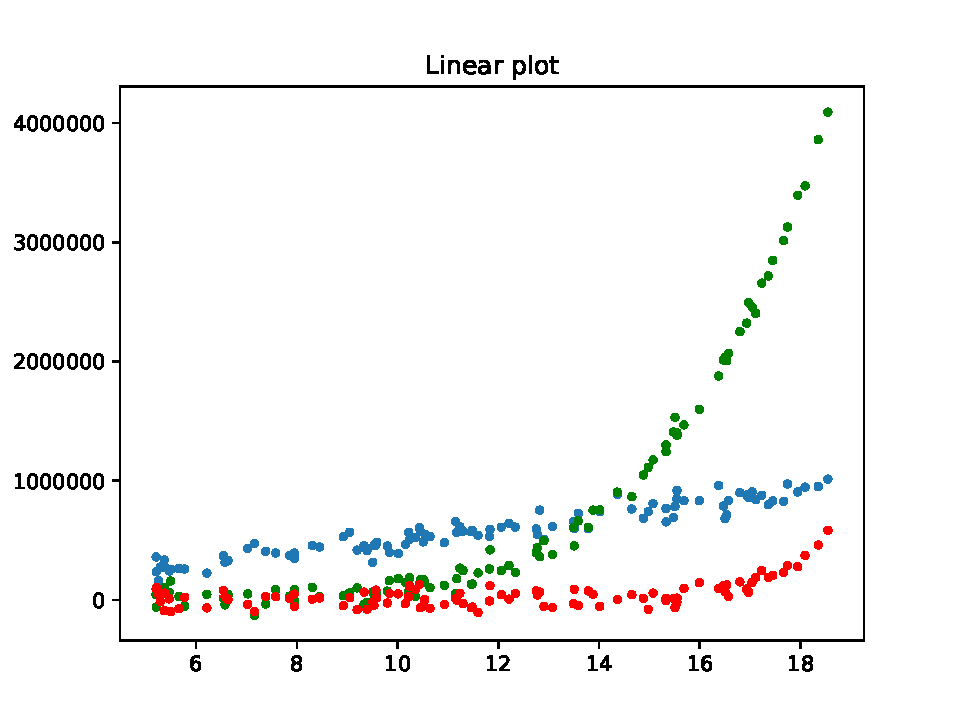
\includegraphics[width=0.6\textwidth,
  alt={Scatter plot titled Linear plot of three synthetic data sets over x from 5 to 18.5, linear vertical axis up to 4 million. Blue points rise slowly along a straight line from about 250,000 to 1 million; green points hug zero until x = 12 and then shoot up past 4 million; red points stay near zero the whole way, reaching only about 600,000 at the far right.}]{logplots1.pdf}
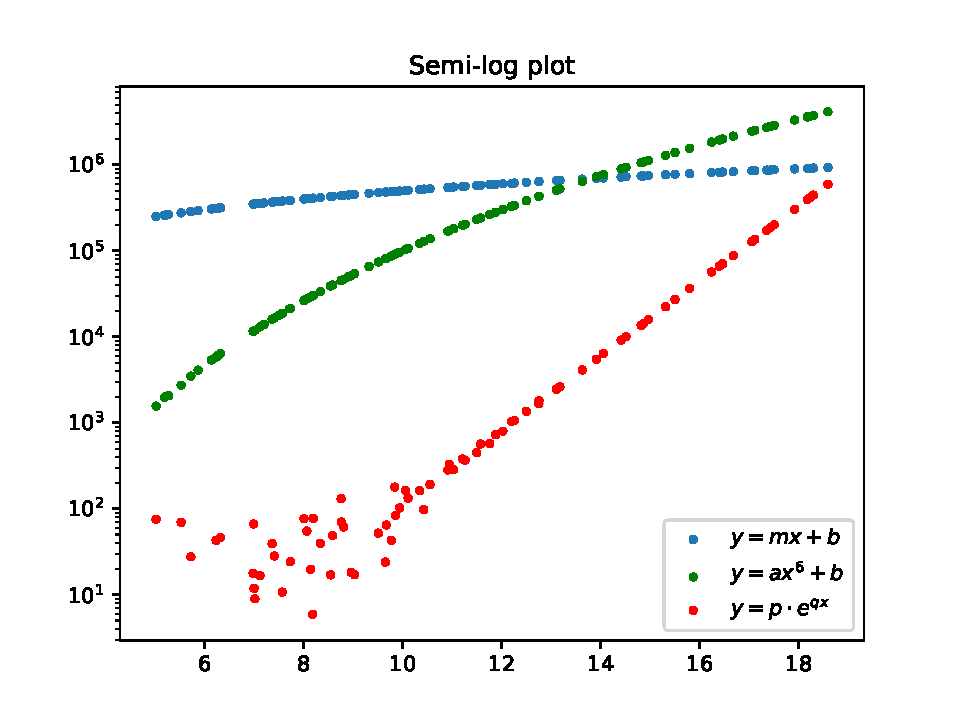
\includegraphics[width=0.6\textwidth,
  alt={Scatter plot titled Semi-log plot of the same three data sets, vertical axis logarithmic from 10 to 10 million, with a legend naming blue y = mx + b, green y = a times x to the sixth plus b, and red y = p times e to the qx. The red exponential points now form a straight line rising from about 10 to 600,000; the green power-law points form a concave-down curve; the blue linear points form a nearly flat, slightly rising curve.}]{logplots2.pdf}
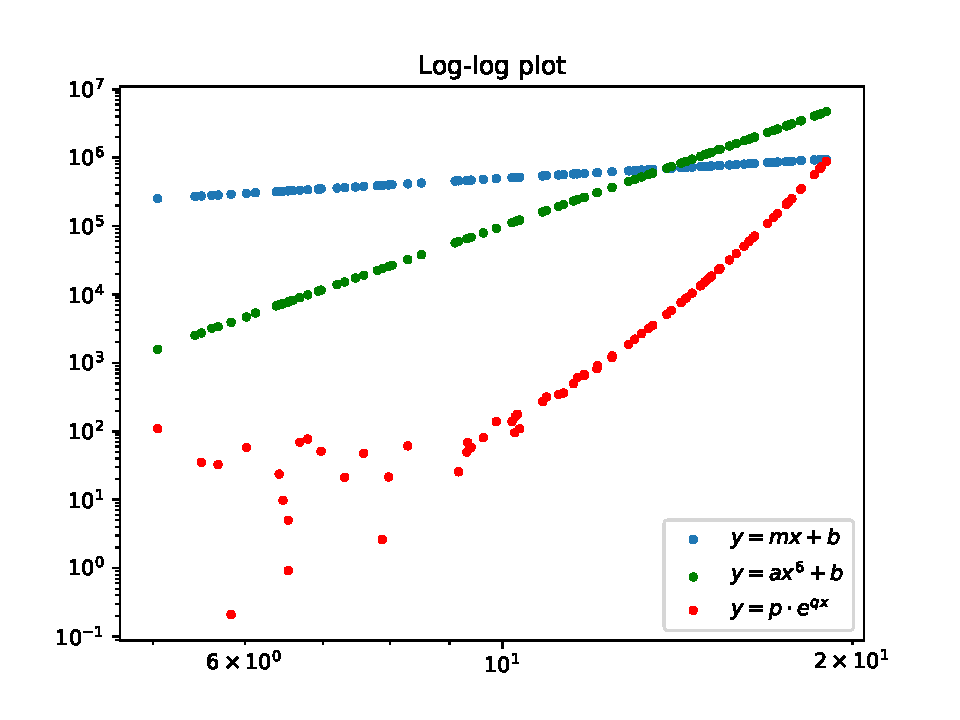
\includegraphics[width=0.6\textwidth,
  alt={Scatter plot titled Log-log plot of the same three data sets, both axes logarithmic. The green power-law points now form a straight line rising from about 1,500 to 5 million; the red exponential points curve upward ever more steeply; the blue linear points form a gently rising curve near the top.}]{logplots3.pdf}
\caption{A linear, semi-log, and log-log plot of the same three data sets:
blue (linear), red (exponential), and green (power-law).}
\label{fig:straightLines}
\end{figure}

In the linear plot, the blue points can be seen to be a straight line. In the
semi-log plot, the red points are. In the log-log plot, the green points are.
This is a powerful tool for recognizing these important kinds of relationships
at a glance.
\end{enumerate}